\section{Gradients and Backpropagation Basics}
\label{sec:gradients-basics}
This section introduces the basic notions of loss functions, gradients, and backpropagation from an abstract operator point of view. In the figures later in the document we mainly show how tensors flow along edges; the detailed Jacobian matrices are not drawn explicitly. Instead, we use a compact notation for local backward operators such as $\mathrm{d}f$, which map upstream gradients on the outputs of a node to gradients on its inputs.

\subsection{Scalar Loss and Gradient Notation}

Training a Transformer model is formulated as minimizing a scalar loss function $\mathcal{L}(\theta)$ with respect to the model parameters $\theta$. For a batch of input--target pairs $(\mathbf{X}, \mathbf{Y}_{\text{targets}})$, the model produces predictions
\[
\mathbf{Y} = f_\theta(\mathbf{X}),
\]
and a scalar loss
\[
\mathcal{L} = \mathcal{L}(\mathbf{Y}, \mathbf{Y}_{\text{targets}}).
\]

We use the differential-style notation $\mathrm{d}\theta = \partial \mathcal{L} / \partial \theta$ for gradients, and we also write $\nabla \theta$ as a shorthand for the same quantity. For example,
\[
  \mathrm{d}\mathbf{X}
  \;=\;
  % \nabla_{\mathbf{X}} \mathcal{L}
  % \;=\;
  \nabla \mathbf{X}
  \;=\;
  \frac{\partial \mathcal{L}}{\partial \mathbf{X}}.
\]

In the diagrams, these gradients appear as edges labeled $\mathrm{d}\mathbf{X}$, $\mathrm{d}\mathbf{W}$, etc. together with their tensor shapes such as $[B, S, D]$ or $[D, D]$.

\subsection{Single-Input Nodes and Backward Operators}

Consider a single node in a computation graph with forward computation
\[
\mathbf{y} = f(\mathbf{x}),
\]
where $\mathbf{x}$ and $\mathbf{y}$ are vectors or tensors. If the loss $\mathcal{L}$ depends on $\mathbf{y}$, then by the chain rule
\[
\mathrm{d}\mathbf{x} = \frac{\partial\mathcal{L}}{\partial\mathbf{x}}
= \frac{\partial\mathcal{L}}{\partial\mathbf{y}} \cdot \frac{\partial\mathbf{y}}{\partial\mathbf{x}}
= \mathrm{d}\mathbf{y} \cdot \frac{\partial f}{\partial\mathbf{x}}.
\]

\textbf{Brief note on Jacobians:} When $\mathbf{x}$ and $\mathbf{y}$ are vectors or tensors, the term $\frac{\partial\mathbf{y}}{\partial\mathbf{x}}$ is formally a \emph{Jacobian matrix} $\mathbf{J}_f(\mathbf{x})$, and the gradient $\mathrm{d}\mathbf{x}$ is computed as a Jacobian-vector product: $\mathrm{d}\mathbf{x} = \mathbf{J}_f(\mathbf{x})^T \mathrm{d}\mathbf{y}$. However, in practice we never materialize the full Jacobian matrix—it would be prohibitively expensive for high-dimensional tensors. Instead, automatic differentiation frameworks directly compute the gradient using efficient chain-rule implementations tailored to each operation.

We introduce an \textbf{abstract backward operator} $\mathrm{d}f$ and write
\[
\boxed{\mathrm{d}\mathbf{x} = \mathrm{d}f(\mathbf{x}, \mathrm{d}\mathbf{y})},
\]
which computes the gradient $\mathrm{d}\mathbf{x}$ given the forward input $\mathbf{x}$ (cached) and the upstream gradient $\mathrm{d}\mathbf{y}$.

\textbf{Graphical representation:}

\begin{center}
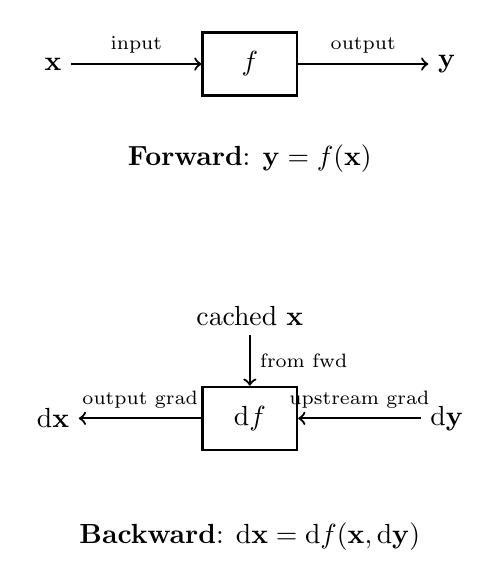
\begin{tikzpicture}[
  node distance=2.5cm,
  fwdnode/.style={rectangle, draw=black, thick, minimum width=1.2cm, minimum height=0.8cm},
  bwdnode/.style={rectangle, draw=black, thick, minimum width=1.2cm, minimum height=0.8cm},
  tensor/.style={},
  arrow/.style={->, thick}
]

% Forward pass
\node[tensor] (x_fwd) {$\mathbf{x}$};
\node[fwdnode, right of=x_fwd, node distance=2.5cm] (f_node) {$f$};
\node[tensor, right of=f_node, node distance=2.5cm] (y_fwd) {$\mathbf{y}$};

\draw[arrow] (x_fwd) -- (f_node) node[midway, above] {\scriptsize input};
\draw[arrow] (f_node) -- (y_fwd) node[midway, above] {\scriptsize output};

\node[below of=f_node, node distance=1.2cm] (fwd_label) {\textbf{Forward}: $\mathbf{y} = f(\mathbf{x})$};

% Backward pass
\node[tensor, below of=x_fwd, node distance=4.5cm] (dx_bwd) {$\mathrm{d}\mathbf{x}$};
\node[bwdnode, right of=dx_bwd, node distance=2.5cm] (df_node) {$\mathrm{d}f$};
\node[tensor, right of=df_node, node distance=2.5cm] (dy_bwd) {$\mathrm{d}\mathbf{y}$};

% Cached input from above
\node[tensor, above of=df_node, node distance=1.3cm] (x_cached) {cached $\mathbf{x}$};

\draw[arrow] (dy_bwd) -- (df_node) node[midway, above] {\scriptsize upstream grad};
\draw[arrow] (df_node) -- (dx_bwd) node[midway, above] {\scriptsize output grad};
\draw[arrow] (x_cached) -- (df_node) node[midway, right] {\scriptsize from fwd};

\node[below of=df_node, node distance=1.5cm] (bwd_label) {\textbf{Backward}: $\mathrm{d}\mathbf{x} = \mathrm{d}f(\mathbf{x}, \mathrm{d}\mathbf{y})$};

\end{tikzpicture}
\end{center}

The diagram shows the key idea: the backward node $\mathrm{d}f$ takes two inputs—the cached forward input $\mathbf{x}$ and the upstream gradient $\mathrm{d}\mathbf{y}$—and produces the output gradient $\mathrm{d}\mathbf{x}$ that flows to the previous layer.

Softmax, dropout, layer normalization, and many other operators in a Transformer layer are special cases of this pattern. Their concrete backward rules are described in terms of such operators $\mathrm{d}f$.

\subsection{Nodes with Multiple Inputs}

Many nodes in a Transformer layer have several inputs. For example, a matrix multiplication node uses both an activation tensor and a weight matrix, and a layer-normalization node uses inputs as well as learned scale and shift parameters. Abstractly, we write
\[
\mathbf{y} = f(\mathbf{x}_1, \mathbf{x}_2, \ldots, \mathbf{x}_k),
\]
where each $\mathbf{x}_i$ may be a tensor of its own.

Given the upstream gradient $\mathrm{d}\mathbf{y} = \partial\mathcal{L}/\partial\mathbf{y}$, the chain rule yields gradients with respect to all inputs:
\[
\mathrm{d}\mathbf{x}_i = \frac{\partial\mathcal{L}}{\partial\mathbf{y}} \cdot \frac{\partial\mathbf{y}}{\partial\mathbf{x}_i} = \mathrm{d}\mathbf{y} \cdot \frac{\partial f}{\partial\mathbf{x}_i}, \quad i = 1, \ldots, k.
\]

We encode this in an abstract backward operator that produces all input gradients simultaneously:
\[
\boxed{(\mathrm{d}\mathbf{x}_1, \ldots, \mathrm{d}\mathbf{x}_k) = \mathrm{d}f(\mathbf{x}_1, \ldots, \mathbf{x}_k, \mathrm{d}\mathbf{y})}.
\]

\subsubsection{Computational Cost: Forward vs. Backward}

\textbf{Can we estimate backward cost from forward cost?} Yes, there are general rules:

\begin{itemize}
\item \textbf{Linear operations (e.g., matrix multiplication):}
\[
\text{Backward cost} \approx 2 \times \text{Forward cost}
\]
For $\mathbf{Y} = \mathbf{X}\mathbf{W}$, the forward pass requires one matmul, while backward requires two: $\mathrm{d}\mathbf{X} = \mathrm{d}\mathbf{Y}\mathbf{W}^T$ and $\mathrm{d}\mathbf{W} = \mathbf{X}^T\mathrm{d}\mathbf{Y}$.

\item \textbf{Element-wise operations (e.g., ReLU, GELU, dropout):}
\[
\text{Backward cost} \approx \text{Forward cost}
\]
For $\mathbf{y} = g(\mathbf{x})$, the backward pass $\mathrm{d}\mathbf{x} = \mathrm{d}\mathbf{y} \odot g'(\mathbf{x})$ has similar complexity to the forward pass.

\item \textbf{Softmax and normalization:}
\[
\text{Backward cost} \approx (1{-}2) \times \text{Forward cost}
\]
The backward pass involves additional dot products or reductions, but remains of the same computational order.

\item \textbf{Attention mechanism:}
\[
\text{Backward cost} \approx 2 \times \text{Forward cost}
\]
Each matmul in forward (e.g., $\mathbf{QK}^T$, attention scores $\times$ $\mathbf{V}$) generates two matmuls in backward.
\end{itemize}

\textbf{Rule of thumb for full networks:}
\[
\boxed{\text{Total backward cost} \approx 2{-}3 \times \text{Total forward cost}}
\]

This factor of 2-3 is why training (forward + backward + optimizer step) takes roughly 3-4$\times$ the time of inference (forward only).

\textbf{Example: Matrix Multiplication}

For matrix multiplication $\mathbf{Y} = \mathbf{X}\mathbf{W}$, the backward pass computes two separate gradients using two matrix multiplications. This separation makes the computational cost and memory usage explicit.

\begin{center}
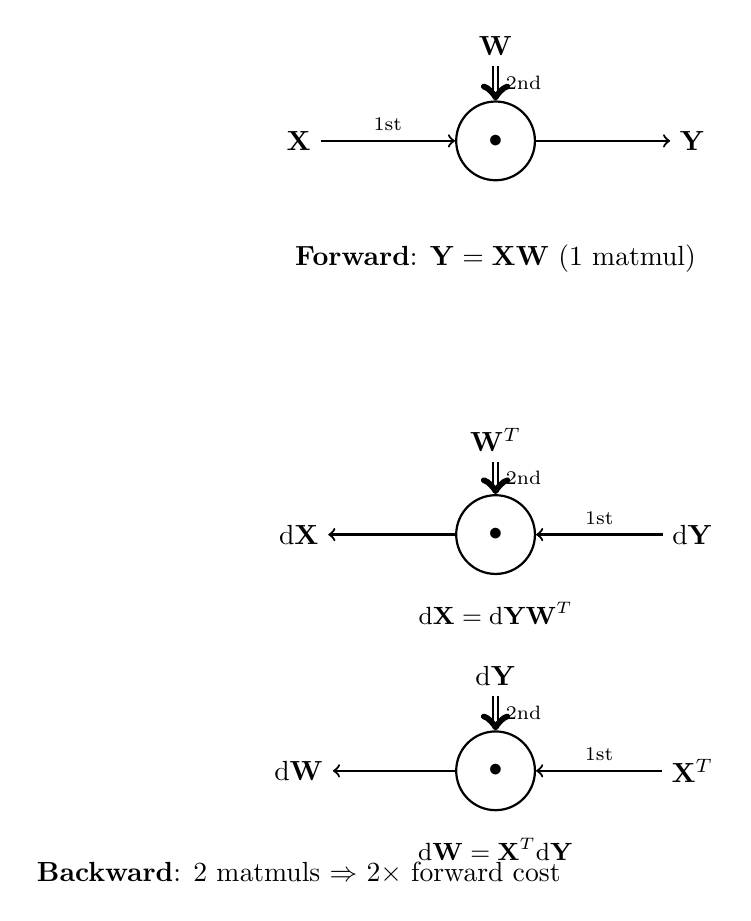
\begin{tikzpicture}[
  node distance=2.5cm,
  fwdnode/.style={circle, draw=black, thick, minimum size=1cm},
  bwdnode/.style={circle, draw=black, thick, minimum size=1cm},
  tensor/.style={},
  arrow/.style={->, thick},
  doublearrow/.style={->, thick, double, double distance=1pt}
]

% Forward pass
\node[tensor] (x_fwd) {$\mathbf{X}$};
\node[fwdnode, right of=x_fwd, node distance=2.5cm] (f_node) {$\bullet$};
\node[tensor, above of=f_node, node distance=1.2cm] (W_fwd) {$\mathbf{W}$};
\node[tensor, right of=f_node, node distance=2.5cm] (y_fwd) {$\mathbf{Y}$};

\draw[arrow] (x_fwd) -- (f_node) node[midway, above] {\scriptsize 1st};
\draw[doublearrow] (W_fwd) -- (f_node) node[midway, right] {\scriptsize 2nd};
\draw[arrow] (f_node) -- (y_fwd);

\node[below of=f_node, node distance=1.5cm] (fwd_label) {\textbf{Forward}: $\mathbf{Y} = \mathbf{X}\mathbf{W}$ (1 matmul)};

% Backward pass - First matmul: dX = dY W^T
\node[tensor, below of=y_fwd, node distance=5cm] (dy_top) {$\mathrm{d}\mathbf{Y}$};
\node[bwdnode, left of=dy_top, node distance=2.5cm] (matmul1) {$\bullet$};
\node[tensor, above of=matmul1, node distance=1.2cm] (WT) {$\mathbf{W}^T$};
\node[tensor, left of=matmul1, node distance=2.5cm] (dx_out) {$\mathrm{d}\mathbf{X}$};

\draw[arrow] (dy_top) -- (matmul1) node[midway, above] {\scriptsize 1st};
\draw[doublearrow] (WT) -- (matmul1) node[midway, right] {\scriptsize 2nd};
\draw[arrow] (matmul1) -- (dx_out);

\node[below of=matmul1, node distance=1.0cm, font=\small] {$\mathrm{d}\mathbf{X} = \mathrm{d}\mathbf{Y}\mathbf{W}^T$};

% Backward pass - Second matmul: dW = X^T dY
\node[tensor, below of=dy_top, node distance=3cm] (XT_right) {$\mathbf{X}^T$};
\node[bwdnode, left of=XT_right, node distance=2.5cm] (matmul2) {$\bullet$};
\node[tensor, above of=matmul2, node distance=1.2cm] (dy_top2) {$\mathrm{d}\mathbf{Y}$};
\node[tensor, left of=matmul2, node distance=2.5cm] (dW_out) {$\mathrm{d}\mathbf{W}$};

\draw[arrow] (XT_right) -- (matmul2) node[midway, above] {\scriptsize 1st};
\draw[doublearrow] (dy_top2) -- (matmul2) node[midway, right] {\scriptsize 2nd};
\draw[arrow] (matmul2) -- (dW_out);

\node[below of=matmul2, node distance=1.0cm, font=\small] {$\mathrm{d}\mathbf{W} = \mathbf{X}^T\mathrm{d}\mathbf{Y}$};

\node[below of=dW_out, node distance=1.3cm] (bwd_label) {\textbf{Backward}: 2 matmuls $\Rightarrow$ 2$\times$ forward cost};

\end{tikzpicture}
\end{center}

\vspace{0.3cm}

\noindent
\textbf{Concrete FLOPs analysis:} For $\mathbf{X} \in \mathbb{R}^{B \times S \times D}$ and $\mathbf{W} \in \mathbb{R}^{D \times D}$:
\begin{align*}
\text{Forward:} \quad & \mathbf{Y} = \mathbf{X}\mathbf{W} \quad \rightarrow \quad 2BSD^2 \text{ FLOPs} \\
\text{Backward:} \quad & \mathrm{d}\mathbf{X} = \mathrm{d}\mathbf{Y}\mathbf{W}^T \quad \rightarrow \quad 2BSD^2 \text{ FLOPs} \\
& \mathrm{d}\mathbf{W} = \mathbf{X}^T\mathrm{d}\mathbf{Y} \quad \rightarrow \quad 2BSD^2 \text{ FLOPs} \\
\text{Total backward:} \quad & 4BSD^2 = 2 \times \text{(forward cost)}
\end{align*}

In the diagrams, we follow the convention that for matrix multiplication nodes:
\begin{itemize}
\item The \textbf{first operand} enters horizontally (from left in forward, from right in backward)
\item The \textbf{second operand} enters vertically from above (shown with a double arrow)
\item The \textbf{output} exits horizontally (to right in forward, to left in backward)
\end{itemize}

This explicit representation allows us to:
\begin{itemize}
\item Count FLOPs precisely for each gradient computation
\item Track memory usage for intermediate tensors
\item Identify opportunities for parallelization (these two matmuls can run in parallel)
\item Match the actual implementation in frameworks like PyTorch and JAX
\end{itemize}

Throughout the document, we follow this convention: whenever the backward pass involves multiple distinct operations, we draw them as separate nodes rather than hiding them inside a single abstract $\mathrm{d}f$ operator.

\subsection{Computation Graph and Backpropagation}

A full Transformer layer can be viewed as a composition of simpler operations:
\[
\mathbf{X}_0 \xrightarrow{f_1} \mathbf{X}_1 \xrightarrow{f_2} \mathbf{X}_2 \xrightarrow{\cdots} \mathbf{X}_L,
\]
where $\mathbf{X}_0$ is the input to the layer and $\mathbf{X}_L$ is the final output before the loss. Each $f_\ell$ is a local operator such as a matrix multiplication, a nonlinearity, a dropout, or a normalization.

Backpropagation proceeds in reverse order. Starting from $\mathrm{d}\mathbf{X}_L = \partial\mathcal{L}/\partial\mathbf{X}_L$, we apply the corresponding backward operator for each node:
\[
\mathrm{d}\mathbf{X}_\ell = \mathrm{d}f_\ell(\mathbf{X}_\ell, \mathrm{d}\mathbf{X}_{\ell+1}), \quad \ell = L-1, L-2, \ldots, 0.
\]

\textbf{Graphical representation of a computation chain:}

\begin{center}
\begin{tikzpicture}[
  node distance=1.8cm,
  fwdnode/.style={rectangle, draw=black, thick, minimum width=1cm, minimum height=0.7cm},
  bwdnode/.style={rectangle, draw=black, thick, minimum width=1cm, minimum height=0.7cm},
  tensor/.style={font=\small},
  arrow/.style={->, thick}
]

% Forward pass
\node[tensor] (x0) {$\mathbf{X}_0$};
\node[fwdnode, right of=x0, node distance=1.8cm] (f1) {$f_1$};
\node[tensor, right of=f1, node distance=1.8cm] (x1) {$\mathbf{X}_1$};
\node[fwdnode, right of=x1, node distance=1.8cm] (f2) {$f_2$};
\node[tensor, right of=f2, node distance=1.8cm] (x2) {$\mathbf{X}_2$};
\node[right of=x2, node distance=0.9cm] (dots) {$\cdots$};
\node[fwdnode, right of=dots, node distance=0.9cm] (fL) {$f_L$};
\node[tensor, right of=fL, node distance=1.8cm] (xL) {$\mathbf{X}_L$};
\node[right of=xL, node distance=1.5cm] (loss) {$\xrightarrow{\mathcal{L}}$};

\draw[arrow] (x0) -- (f1);
\draw[arrow] (f1) -- (x1);
\draw[arrow] (x1) -- (f2);
\draw[arrow] (f2) -- (x2);
\draw[arrow] (x2) -- (dots);
\draw[arrow] (dots) -- (fL);
\draw[arrow] (fL) -- (xL);

\node[above of=x1, node distance=0.9cm] {\scriptsize\textbf{Forward pass}};

% Backward pass
\node[tensor, below of=x0, node distance=3.5cm] (dx0) {$\mathrm{d}\mathbf{X}_0$};
\node[bwdnode, right of=dx0, node distance=1.8cm] (df1) {$\mathrm{d}f_1$};
\node[tensor, right of=df1, node distance=1.8cm] (dx1) {$\mathrm{d}\mathbf{X}_1$};
\node[bwdnode, right of=dx1, node distance=1.8cm] (df2) {$\mathrm{d}f_2$};
\node[tensor, right of=df2, node distance=1.8cm] (dx2) {$\mathrm{d}\mathbf{X}_2$};
\node[right of=dx2, node distance=0.9cm] (bdots) {$\cdots$};
\node[bwdnode, right of=bdots, node distance=0.9cm] (dfL) {$\mathrm{d}f_L$};
\node[tensor, right of=dfL, node distance=1.8cm] (dxL) {$\mathrm{d}\mathbf{X}_L$};

\draw[arrow] (dx1) -- (df1);
\draw[arrow] (df1) -- (dx0);
\draw[arrow] (dx2) -- (df2);
\draw[arrow] (df2) -- (dx1);
\draw[arrow] (bdots) -- (dx2);
\draw[arrow] (dxL) -- (dfL);
\draw[arrow] (dfL) -- (bdots);

\node[above of=dx1, node distance=0.9cm] {\scriptsize\textbf{Backward pass}};

% Cached inputs from above
\node[tensor, above of=df1, node distance=1.1cm, font=\tiny] (x0_cached) {$\mathbf{X}_0$};
\node[tensor, above of=df2, node distance=1.1cm, font=\tiny] (x1_cached) {$\mathbf{X}_1$};
\node[tensor, above of=dfL, node distance=1.1cm, font=\tiny] (xL_cached) {$\mathbf{X}_{L-1}$};

\draw[arrow] (x0_cached) -- (df1);
\draw[arrow] (x1_cached) -- (df2);
\draw[arrow] (xL_cached) -- (dfL);

\end{tikzpicture}
\end{center}

\vspace{0.3cm}

\noindent
Key observations:
\begin{itemize}
\item \textbf{Forward}: Data flows left to right through function nodes $f_\ell$
\item \textbf{Backward}: Gradients flow right to left through backward nodes $\mathrm{d}f_\ell$
\item \textbf{Cache}: Each backward node $\mathrm{d}f_\ell$ receives the cached forward state from above
\item \textbf{Chain rule}: $\mathrm{d}\mathbf{X}_\ell = \mathrm{d}f_\ell(\mathbf{X}_\ell, \mathrm{d}\mathbf{X}_{\ell+1})$ for $\ell = L-1, \ldots, 0$
\end{itemize}

If $f_\ell$ depends on additional inputs (e.g. parameters), then its backward operator also produces gradients with respect to those inputs, as discussed below.

In the diagrams, we emphasize this process by drawing:
\begin{itemize}
\item \textbf{forward edges} for $\mathbf{X}_\ell$ flowing into the forward nodes $f_\ell$,
\item \textbf{backward edges} for $\mathrm{d}\mathbf{X}_\ell$ flowing out of the corresponding backward nodes $\mathrm{d}f_\ell$.
\end{itemize}

The detailed formulas that define each local operator $\mathrm{d}f_\ell$ are hidden inside the node and explained in the operator dictionary of Section 4.

\subsection{Parameter Gradients and Updates}

Parameters such as weight matrices and bias vectors enter the graph as additional inputs to some node. For example, consider a matrix multiplication
\[
\mathbf{Y} = \mathbf{X}\mathbf{W},
\]
where $\mathbf{X}$ is an activation tensor and $\mathbf{W}$ is a weight matrix. We view this as a function of two inputs,
\[
\mathbf{Y} = f(\mathbf{X}, \mathbf{W}).
\]

The corresponding backward operator produces both activation and parameter gradients:
\[
\boxed{(\mathrm{d}\mathbf{X}, \mathrm{d}\mathbf{W}) = \mathrm{d}f(\mathbf{X}, \mathbf{W}, \mathrm{d}\mathbf{Y})}.
\]

\textbf{Parameter gradient flow:}

\begin{center}
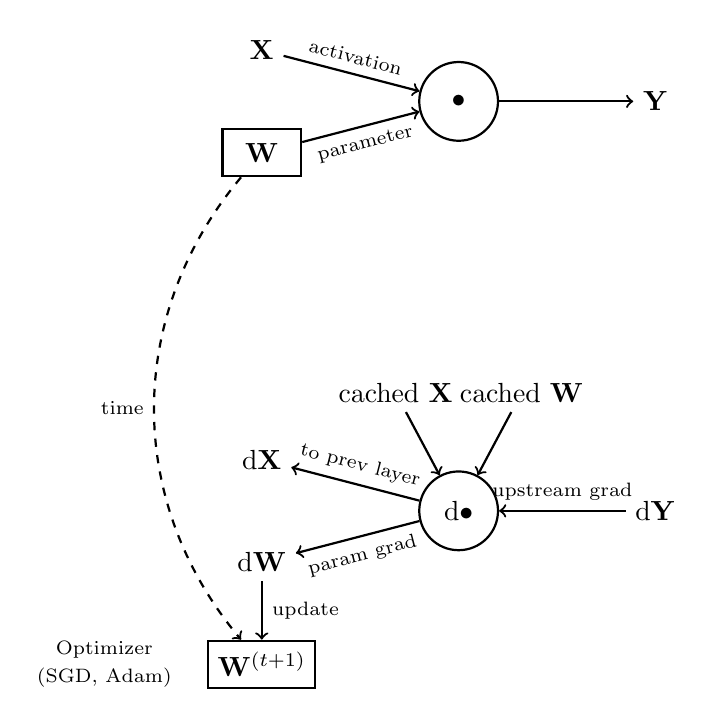
\begin{tikzpicture}[
  node distance=2.2cm,
  fwdnode/.style={circle, draw=black, thick, minimum size=1cm},
  bwdnode/.style={circle, draw=black, thick, minimum size=1cm},
  paramnode/.style={rectangle, draw=black, thick, minimum width=1cm, minimum height=0.6cm},
  tensor/.style={},
  arrow/.style={->, thick}
]

% Forward pass
\node[tensor] (x_fwd) {$\mathbf{X}$};
\node[paramnode, below of=x_fwd, node distance=1.3cm] (W_fwd) {$\mathbf{W}$};
\node[fwdnode, right of=x_fwd, yshift=-0.65cm, node distance=2.5cm] (f_node) {$\bullet$};
\node[tensor, right of=f_node, node distance=2.5cm] (y_fwd) {$\mathbf{Y}$};

\draw[arrow] (x_fwd) -- (f_node) node[midway, above, sloped] {\scriptsize activation};
\draw[arrow] (W_fwd) -- (f_node) node[midway, below, sloped] {\scriptsize parameter};
\draw[arrow] (f_node) -- (y_fwd);

% Backward pass
\node[tensor, below of=x_fwd, node distance=5.2cm] (dx_bwd) {$\mathrm{d}\mathbf{X}$};
\node[tensor, below of=W_fwd, node distance=5.2cm] (dW_bwd) {$\mathrm{d}\mathbf{W}$};
\node[bwdnode, right of=dx_bwd, yshift=-0.65cm, node distance=2.5cm] (df_node) {$\mathrm{d}\bullet$};
\node[tensor, right of=df_node, node distance=2.5cm] (dy_bwd) {$\mathrm{d}\mathbf{Y}$};

% Cached inputs from above
\node[tensor, above of=df_node, node distance=1.5cm, xshift=-0.8cm] (x_cached) {cached $\mathbf{X}$};
\node[tensor, above of=df_node, node distance=1.5cm, xshift=0.8cm] (W_cached) {cached $\mathbf{W}$};

\draw[arrow] (dy_bwd) -- (df_node) node[midway, above] {\scriptsize upstream grad};
\draw[arrow] (df_node) -- (dx_bwd) node[midway, above, sloped] {\scriptsize to prev layer};
\draw[arrow] (df_node) -- (dW_bwd) node[midway, below, sloped] {\scriptsize param grad};
\draw[arrow] (x_cached) -- (df_node);
\draw[arrow] (W_cached) -- (df_node);

% Optimizer
\node[paramnode, below of=dW_bwd, node distance=1.3cm] (W_next) {$\mathbf{W}^{(t+1)}$};
\node[left of=W_next, node distance=2cm, align=center] (opt_label) {\scriptsize Optimizer\\[-2pt]\scriptsize (SGD, Adam)};

\draw[arrow] (dW_bwd) -- (W_next) node[midway, right] {\scriptsize update};
\draw[arrow, dashed, bend right=40] (W_fwd) to node[midway, left] {\scriptsize time} (W_next);

\end{tikzpicture}
\end{center}

\vspace{0.3cm}

\noindent
An optimizer then uses the parameter gradients to update the parameters. For example, stochastic gradient descent with learning rate $\eta$ performs
\[
\theta^{(t+1)} = \theta^{(t)} - \eta \, \mathrm{d}\theta^{(t)}.
\]

\textbf{Key distinction}:
\begin{itemize}
\item \textbf{Activation gradients} ($\mathrm{d}\mathbf{X}$): Flow to the previous layer in the backward pass
\item \textbf{Parameter gradients} ($\mathrm{d}\mathbf{W}$): Accumulated and used by the optimizer to update weights
\end{itemize}

In this document we do not draw optimizer steps in the diagrams; we only show how $\mathrm{d}\mathbf{W}$ and $\mathrm{d}\mathbf{b}$ are computed by the backward nodes.

\subsection{Connection to the Diagrams}

The detailed MHA, MLP, and output-projection figures in later sections are best read with this abstract picture in mind:
\begin{itemize}
\item Each \textbf{forward node} (e.g. \texttt{SM}, \texttt{S}, \texttt{DO}, \texttt{LN}, \texttt{matmul}) represents a mapping $\mathbf{y} = f(\mathbf{x}_1, \ldots, \mathbf{x}_k)$.
\item Each corresponding \textbf{backward node} (e.g. \texttt{dSM}, \texttt{dS}, \texttt{dDO}, \texttt{dLN}, \texttt{dMatmul}) represents the operator
\[
(\mathrm{d}\mathbf{x}_1, \ldots, \mathrm{d}\mathbf{x}_k) = \mathrm{d}f(\mathbf{x}_1, \ldots, \mathbf{x}_k, \mathrm{d}\mathbf{y}),
\]
implemented using the appropriate Jacobian-transpose formulas for that operator.
\item Edges labeled with tensors such as $\mathbf{X}$, $\mathbf{H}$, $\mathbf{Q}$, $\mathbf{K}$, $\mathbf{V}$, $\mathbf{AS}$, and their gradients $\mathrm{d}\mathbf{X}$, $\mathrm{d}\mathbf{Q}$, $\mathrm{d}\mathbf{W}$, etc., capture only the flow of data, together with compact shape annotations like $[B, S, D]$ or $[B, N_H, S, D_h]$.
\end{itemize}

In the next section we define the graphical notation and operator dictionary used in the figures, and we specialize the abstract backward operator $\mathrm{d}f$ to concrete nodes such as softmax (\texttt{S}/\texttt{dS}), scale/mask (\texttt{SM}/\texttt{dSM}), dropout (\texttt{DO}/\texttt{dDO}), and layer normalization (\texttt{LN}/\texttt{dLN}).